\documentclass[a4paper,12pt]{article}
\usepackage{latexsym}
\usepackage{graphicx}
\usepackage{epsfig}
\usepackage{float}
\usepackage{natbib}
\usepackage{listings}
\usepackage[skip=0pt]{caption}
\graphicspath{{./}}
\DeclareGraphicsExtensions{.eps}
%\setlength\abovecaptionskip{-5pt}
\author{Howard Kinsman}
\title{MSc Project - Modelling a Double Barred Galaxy as a Double Binary}
\begin{document}
\maketitle
\section{Introduction}
The aim of this project was to create a simple model of a double barred galaxy using a double binary.

\section{Methods}
Fortran 90 was selected as the language of choice in order to avoid the fixed line limitations of Fortran 77.
The model was created using OdeInt from Numerical Recipes. I first converted OdeInt to Fortran 90 for this purpose.
Please see the Compilers subsection for a few notes on compilers - may or may not be relevant to the project.
\newline
The classical equations of motion for an n-body problem are:
\begin{equation}
m_i\mathbf{\ddot{r}}=\sum_{i\neq{j}}\frac{{m_i}{m_j}}{r^3_{ij}}\mathbf{r_{ij}}
\qquad
i=1,2,3...
\end{equation}
where $\mathbf{r_i}=\left(x_i,y_i\right)$ and $\mathbf{r_{ij}}=\mathbf{r_j}-\mathbf{r_i}$. So for a four body problem 
this equation results in the following:
\begin{equation}
\ddot{\mathbf{r_1}}=\frac{m_2\mathbf{r}_{12}}{r^3_{12}}+\frac{m_3\mathbf{r}_{13}}{r^3_{13}}+\frac{m_4\mathbf{r}_{14}}{r^3_{14}}
\end{equation}
\begin{equation}
\ddot{\mathbf{r_2}}=\frac{m_1\mathbf{r}_{21}}{r^3_{21}}+\frac{m_3\mathbf{r}_{23}}{r^3_{23}}+\frac{m_4\mathbf{r}_{24}}{r^3_{24}}
\end{equation}
\begin{equation}
\ddot{\mathbf{r_3}}=\frac{m_1\mathbf{r}_{31}}{r^3_{31}}+\frac{m_2\mathbf{r}_{32}}{r^3_{32}}+\frac{m_4\mathbf{r}_{34}}{r^3_{34}}
\end{equation}
\begin{equation}
\ddot{\mathbf{r_4}}=\frac{m_1\mathbf{r}_{41}}{r^3_{41}}+\frac{m_2\mathbf{r}_{42}}{r^3_{42}}+\frac{m_3\mathbf{r}_{43}}{r^3_{43}}
\end{equation}
The above equations were encoded into Fortran. A full code listing is supplied in a separate file.
\subsection{Initial Conditions}
As a starting point both the outer binary and inner binary were placed in circular orbits and tested separately and then combined to ensure a stable
starting point. The inner binary had initially a neglible mass.
The outer binary initial conditions were:
\begin{lstlisting}
m1=.5, m2=.5, x1=-.5, x2=.5, y1=0, y2=0,
vx1=0, vx2=0, vy1=-.5, vy2=.5
\end{lstlisting}
and for the inner binary:
\begin{lstlisting}
m3=.001, m3=.001, x3=-.001, x4=.001, y3=0, y4=0, 
vx3=0, vx4=0, vy3=-.5, vy4=.5
\end{lstlisting}
Plots of the two initial binaries are shown in Fig. \ref{fig:outerbinary} and 
\ref{fig:innerbinary}. The scale of the inner binary is so small that it is difficult
to see in GnuPlot.
\begin{figure}[H]
\centering
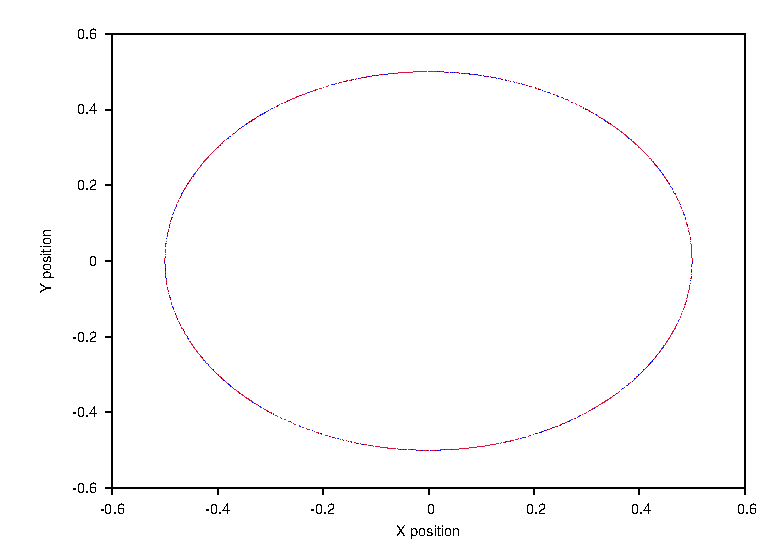
\includegraphics[width=.9\textwidth]{./results/outerbinary/Orbit.eps}
\caption{Outer Binary}
\label{fig:outerbinary}
\end{figure}
\begin{figure}[H]
\centering
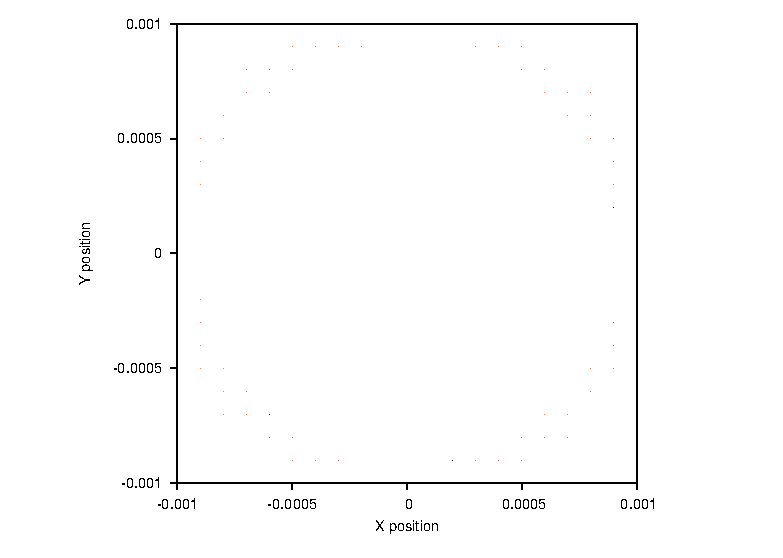
\includegraphics[width=.9\textwidth]{./results/innerbinary/Orbit.eps}
\caption{Inner Binary}
\label{fig:innerbinary}
\end{figure}
I then proceeded to perturb the system by gradually increasing the mass of the inner binary. As the system became unstable I componensated for
the increasing mass of the inner binary by increasing the velocity of the outer binary and also decreasing the velocity and increasing the binary 
separation of the inner binary. In many of the configurations the systems were inherently unstable and produced collisions with some 
or all of the bodies being ejected from the system. These were rejected and only 'stable' configurations were considered.
Table \ref{tab:variables} shows the perturbations made to the system - only the variables in this table changed and all the other initial
conditions remained the same.
\begin{table}[ht!]
  \centering
  \caption{Configurations}
  \label{tab:variables}
  \begin{tabular}{ccccccccc}
   Config. & m3 & m4 & vy1 & vy2 & x3 & x4 & vy3 & vy4\\
    \hline
   1 & .001 & .001 & -.5 & .5 & -.001 & .001 & -.5 & .5\\
   2 & .002 & .002 & -.5 & .5 & -.001 & .001 & -.5 & .5\\
   3 & .003 & .003 & -.5 & .5 & -.001 & .001 & -.5 & .5\\
   4 & .004 & .004 & -.5 & .5 & -.004 & .004 & -.5 & .5\\
   5 & .004 & .004 & -.55 & .55 & -.004 & .004 & -.5 & .5\\
   6 & .004 & .004 & -.57 & .57 & -.004 & .004 & -.5 & .5\\
   7 & .005 & .005 & -.58 & .58 & -.005 & .005 & -.3 & .3\\
   8 & .005 & .005 & -.58 & .58 & -.005 & .005 & -.4 & .4\\
   9 & .005 & .005 & -.58 & .58 & -.005 & .005 & -.35 & .35\\
   10 & .006 & .006 & -.6 & .6 & -.006 & .006 & -.3 & .3\\
   11 & .01 & .01 & -.7 & .7 & -.01 & .01 & -.2 & .2\\
   12 & .02 & .02 & -.75 & .75 & -.02 & .02 & -.1 & .1\\
   13 & .025 & .025 & -.65 & .65 & -.02 & .02 & -.5 & .5\\
   14 & .05 & .05 & -.9 & .9 & -.05 & .05 & -.1 & .1\\
   15 & .05 & .05 & -.9 & .9 & -.05 & .05 & -.15 & .15\\
   16 & .06 & .06 & -.95 & .95 & -.06 & .06 & -.15 & .15\\
   17 & .07 & .07 & -.1 & .1 & -.07 & .07 & -.15 & .15\\
   18 & .08 & .08 & -.105 & .105 & -.08 & .08 & -.12 & .12\\
  \end{tabular}
\end{table}
\subsection{Compilers}
As I had converted OdeInt into Fortran 90 I wanted to make sure I hadn't introduced any errors. I therefore compared the output of the Numerical Recipes
version of OdeInt with mine. I was compiling with GFortran and the Fortran 77 version was compiled with g77. They were different! So naturally concerned 
I then compiled the Fortran 77 version with GFortran. The results were identical to mine, which satisified me that I hadn't introduced any errors.

\section{Results}
As can be seen from Fig. \ref{fig:config1} even a neglible mass inner binary causes the outer binary to begin to separate and become less tightly bound.
Figures Fig. \ref{fig:config1} to \ref{fig:config18i} show plots of the double binary using the parameters given in Table \ref{tab:variables}.
In many cases the inner binary is only visible as a point at the centre of the outer binary.
As the mass of the inner binary increased the system became increasingly unstablle and the effect on the outer binary became more pronounced.
Even the 'stable' configurations listed in Table \ref{tab:variables} hold for only a few orbits.
I was unable to recreate a stable system for a mass $>.08$ for the inner bar.
The plots below reveal that increasing the mass of the inner binary causes the outer binary to separate and
form wider orbits.
\begin{figure}[H]
\centering
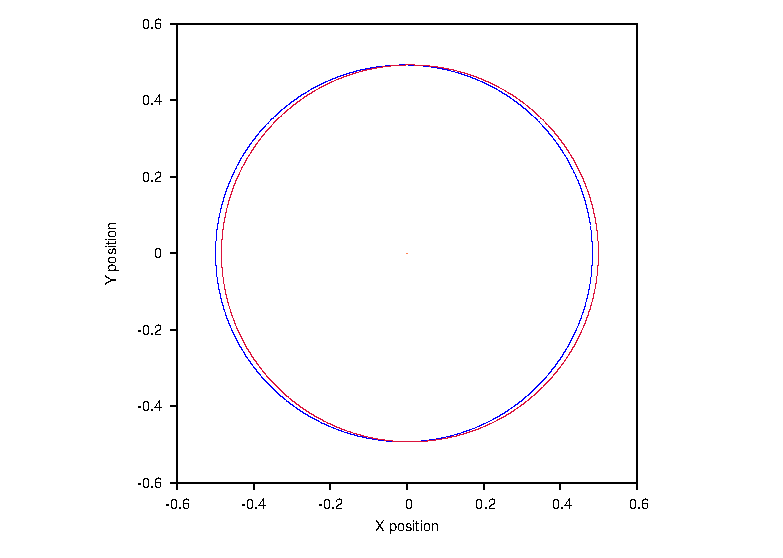
\includegraphics[width=.9\textwidth]{./results/stablebase/Orbit.eps}
\caption{Configuration 1}
\label{fig:config1}
\end{figure}

\begin{figure}[H]
\centering
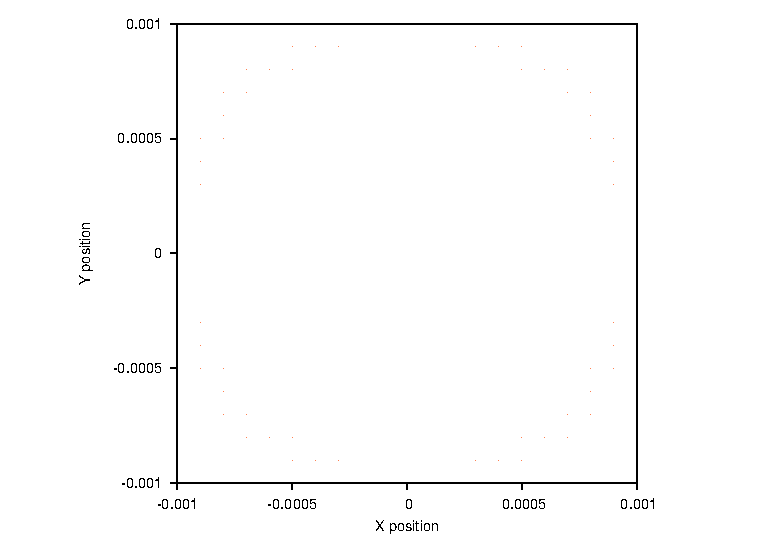
\includegraphics[width=.9\textwidth]{./results/stablebase/Inner.eps}
\caption{Configuration 1 - Inner Bar}
\label{fig:config1i}
\end{figure}

\begin{figure}[H]
\centering
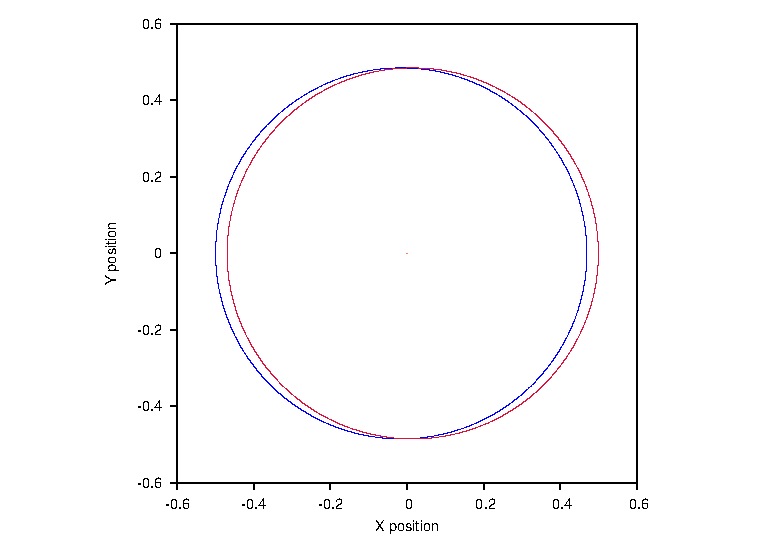
\includegraphics[width=.9\textwidth]{./results/002-5-001/Orbit.eps}
\caption{Configuration 2}
\label{fig:config2}
\end{figure}

\begin{figure}[H]
\centering
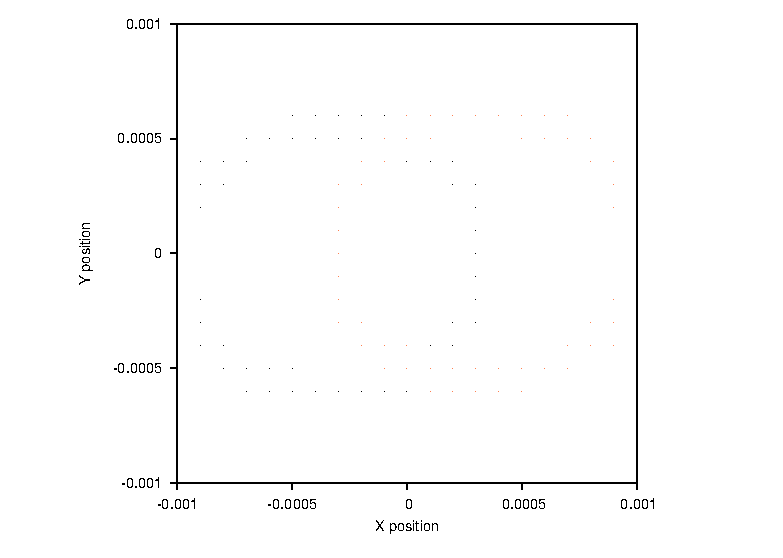
\includegraphics[width=.9\textwidth]{./results/002-5-001/Inner.eps}
\caption{Configuration 2 - Inner Bar}
\label{fig:config2i}
\end{figure}

\begin{figure}[H]
\centering
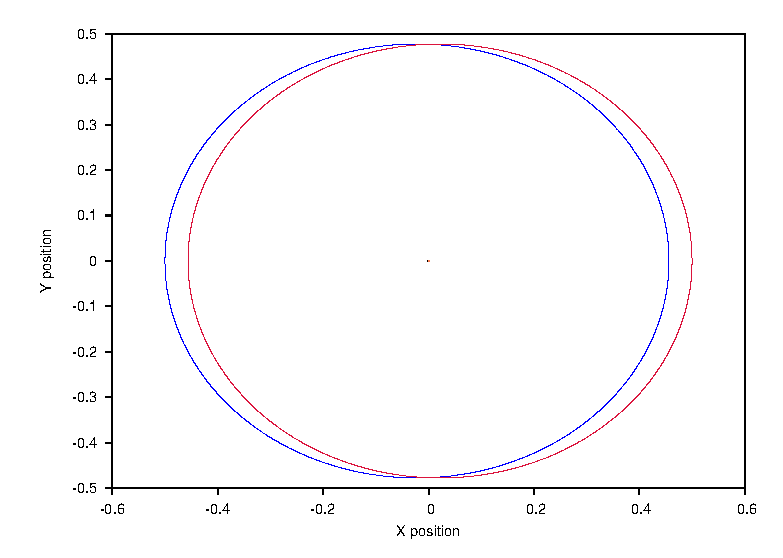
\includegraphics[width=.9\textwidth]{./results/003-5-001/Orbit.eps}
\caption{Configuration 3}
\label{fig:config3}
\end{figure}
\begin{figure}[H]
\centering
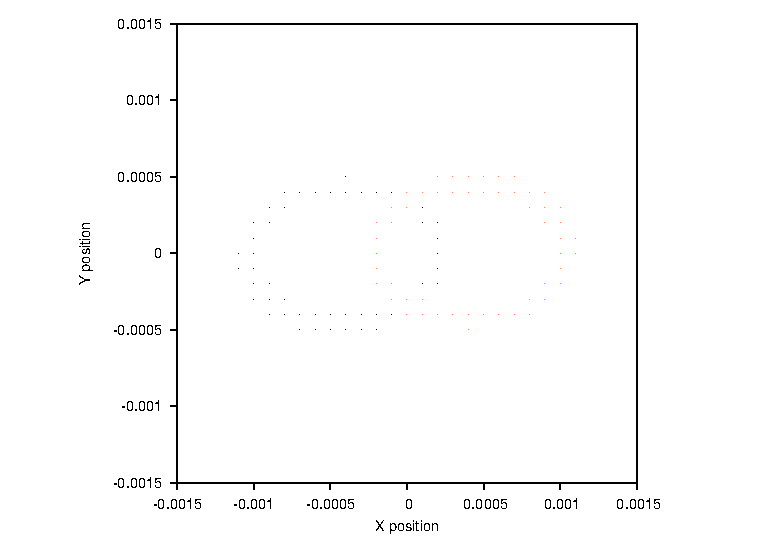
\includegraphics[width=.9\textwidth]{./results/003-5-001/Inner.eps}
\caption{Configuration 3 - Inner Bar}
\label{fig:config3i}
\end{figure}

\begin{figure}[H]
\centering
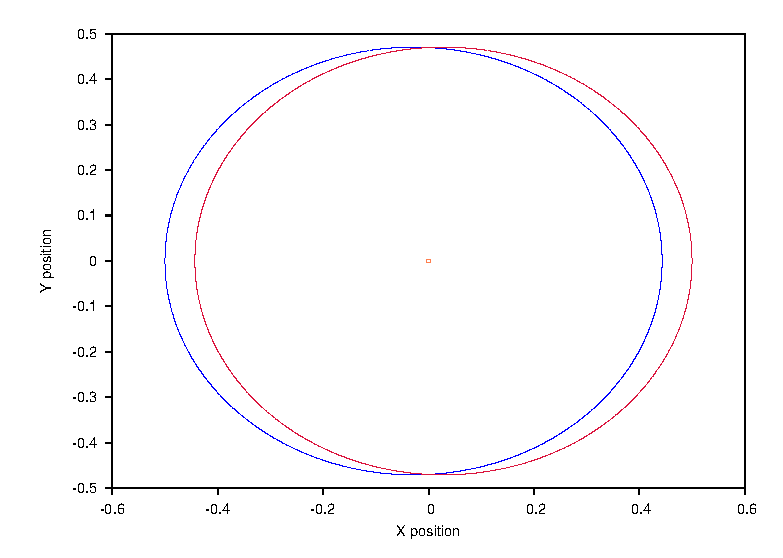
\includegraphics[width=0.9\textwidth]{./results/004-5-004/Orbit.eps}
\caption{Configuration 4}
\label{fig:config4}
\end{figure}
\begin{figure}[H]
\centering
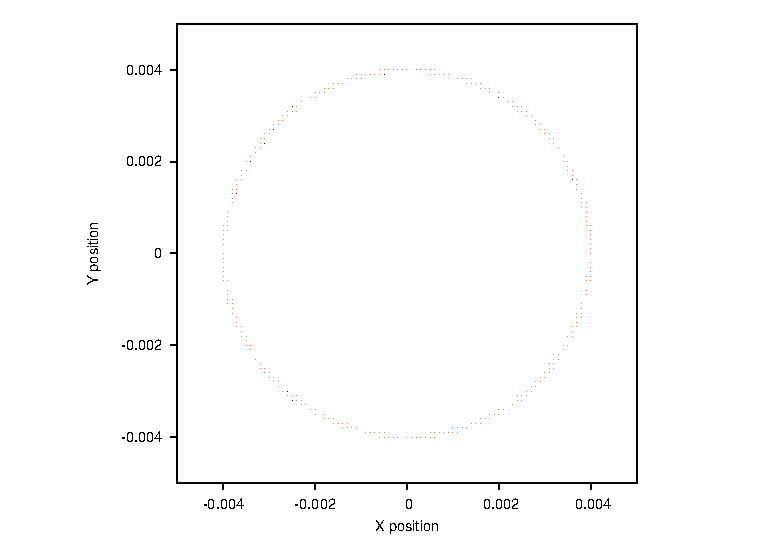
\includegraphics[width=0.9\textwidth]{./results/004-5-004/Inner.eps}
\caption{Configuration 4 - Inner Bar}
\label{fig:config4i}
\end{figure}

\begin{figure}[H]
\centering
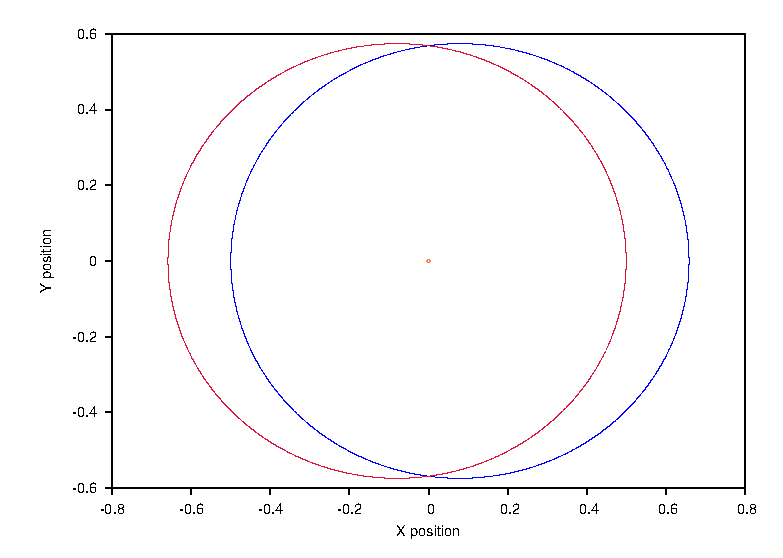
\includegraphics[width=0.9\textwidth]{./results/004-55-004/Orbit.eps}
\caption{Configuration 5}
\label{fig:config5}
\end{figure}
\begin{figure}[H]
\centering
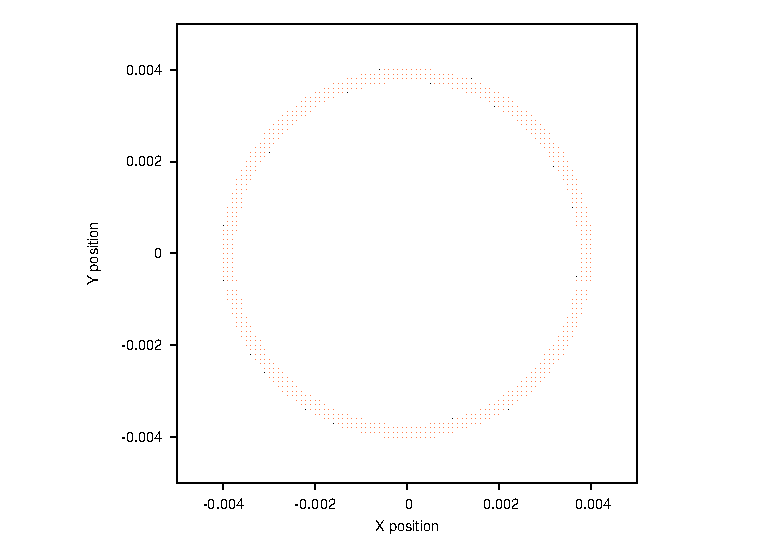
\includegraphics[width=0.9\textwidth]{./results/004-55-004/Inner.eps}
\caption{Configuration 5 - Inner Bar}
\label{fig:config5i}
\end{figure}

\begin{figure}[H]
\centering
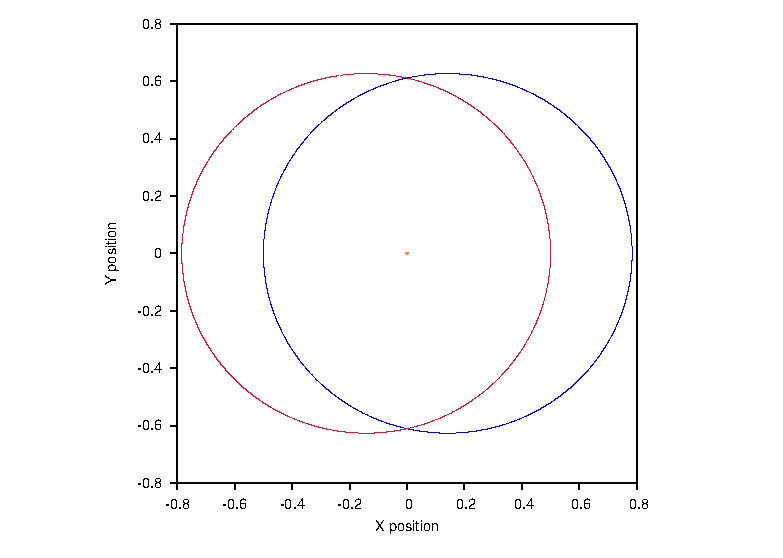
\includegraphics[width=0.9\textwidth]{./results/004-57-004/Orbit.eps}
\caption{Configuration 6}
\label{fig:config6}
\end{figure}
\begin{figure}[H]
\centering
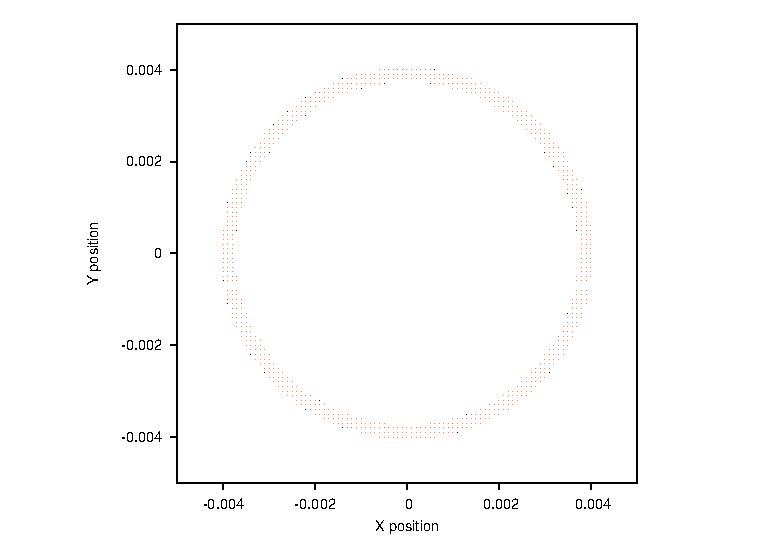
\includegraphics[width=0.9\textwidth]{./results/004-57-004/Inner.eps}
\caption{Configuration 6 - Inner Bar}
\label{fig:config6i}
\end{figure}

\begin{figure}[H]
\centering
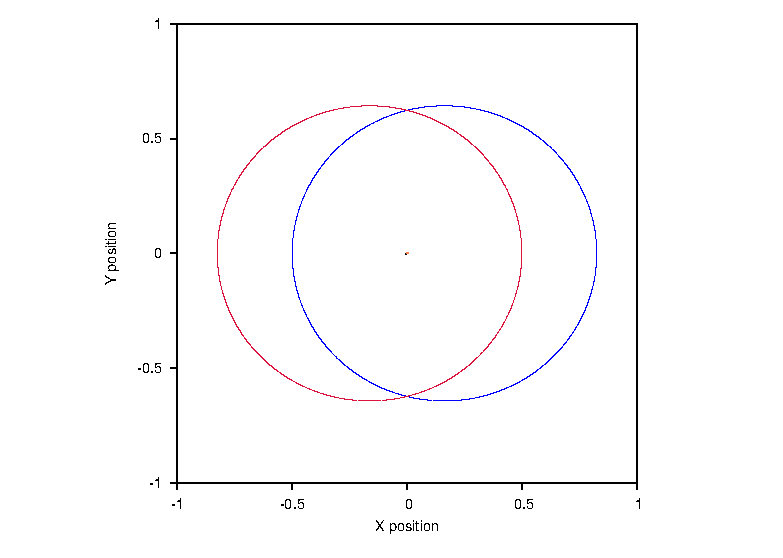
\includegraphics[width=0.9\textwidth]{./results/005-58-005-3/Orbit.eps}
\caption{Configuration 7}
\label{fig:config7}
\end{figure}
\begin{figure}[H]
\centering
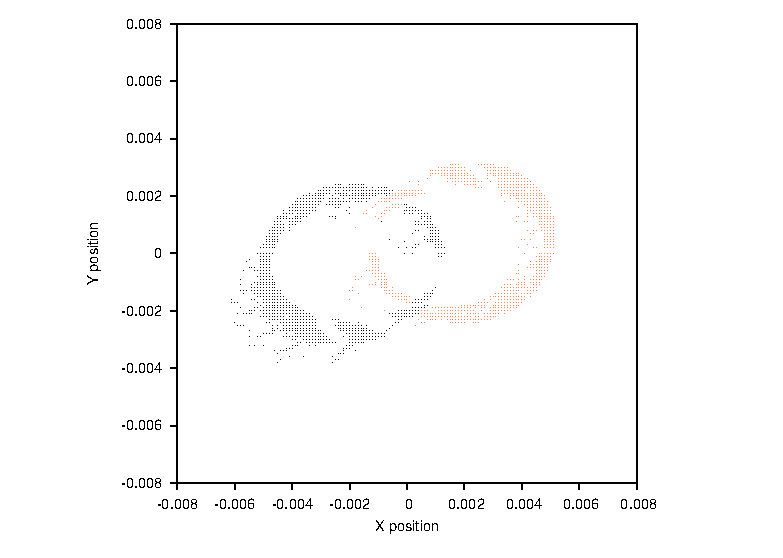
\includegraphics[width=0.9\textwidth]{./results/005-58-005-3/Inner.eps}
\caption{Configuration 7 - Inner Bar}
\label{fig:config7i}
\end{figure}

\begin{figure}[H]
\centering
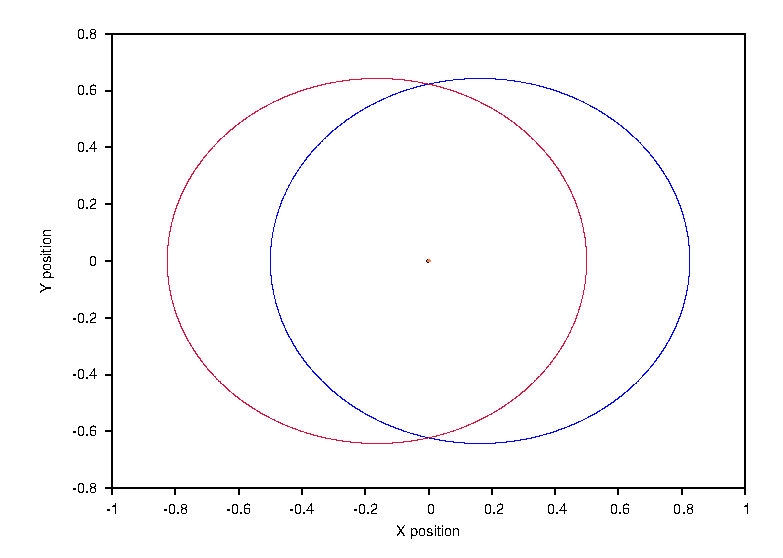
\includegraphics[width=0.9\textwidth]{./results/005-58-005-4/Orbit.eps}
\caption{Configuration 8}
\label{fig:config8}
\end{figure}
\begin{figure}[H]
\centering
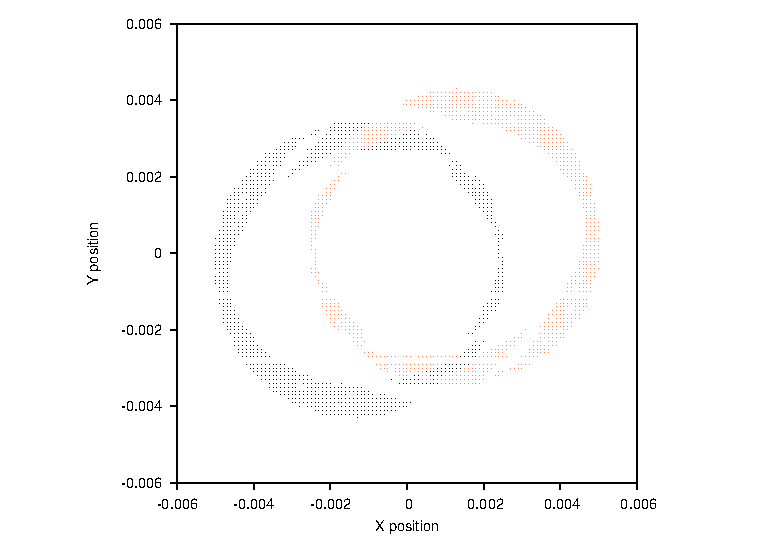
\includegraphics[width=0.9\textwidth]{./results/005-58-005-4/Inner.eps}
\caption{Configuration 8 - Inner Bar}
\label{fig:config8i}
\end{figure}

\begin{figure}[H]
\centering
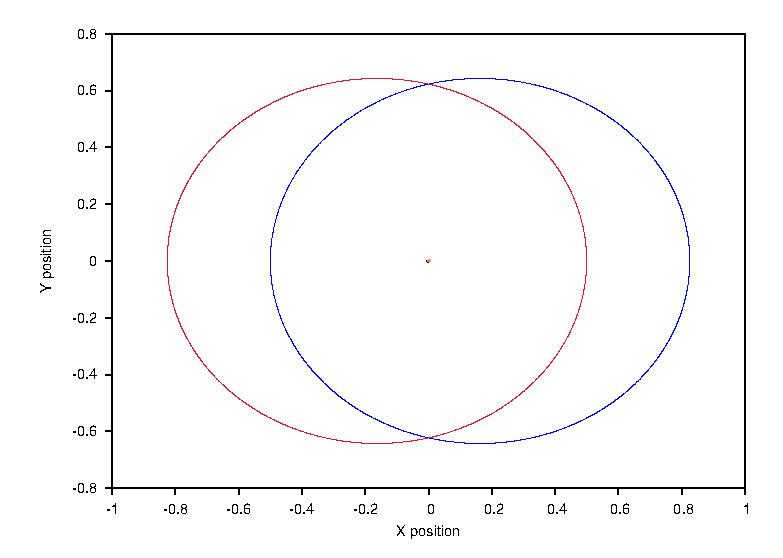
\includegraphics[width=0.9\textwidth]{./results/005-58-005-35/Orbit.eps}
\caption{Configuration 9}
\label{fig:config9}
\end{figure}
\begin{figure}[H]
\centering
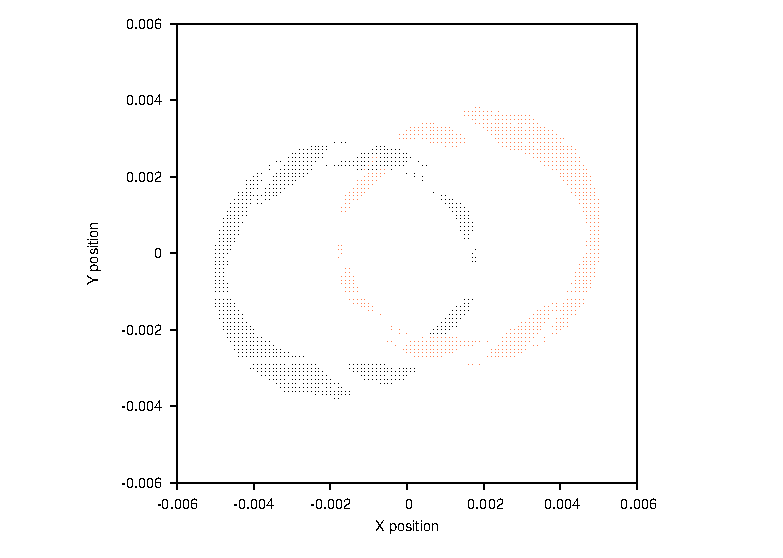
\includegraphics[width=0.9\textwidth]{./results/005-58-005-35/Inner.eps}
\caption{Configuration 9 - Inner Bar}
\label{fig:config9i}
\end{figure}

\begin{figure}[H]
\centering
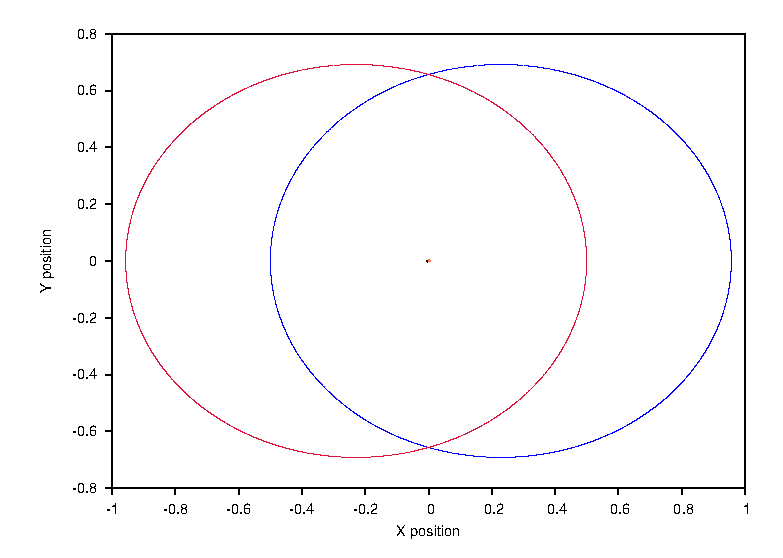
\includegraphics[width=0.9\textwidth]{./results/006-6-006-3/Orbit.eps}
\caption{Configuration 10}
\label{fig:config10}
\end{figure}
\begin{figure}[H]
\centering
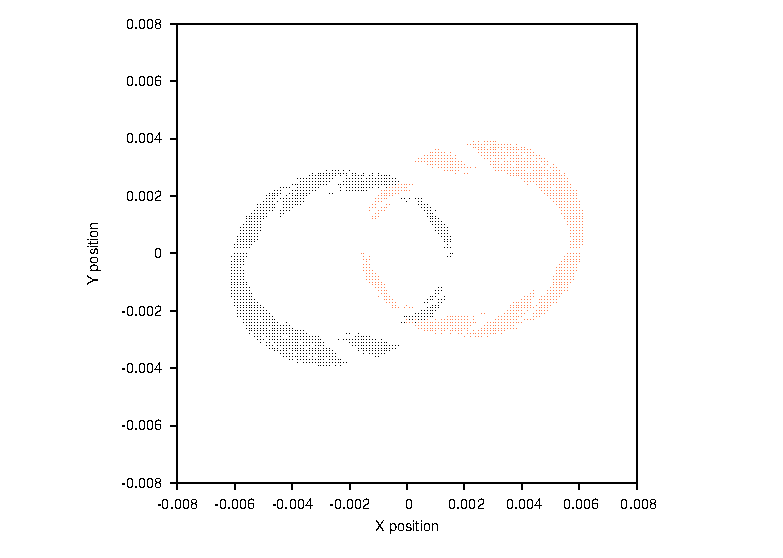
\includegraphics[width=0.9\textwidth]{./results/006-6-006-3/Inner.eps}
\caption{Configuration 10 - Inner Bar}
\label{fig:config10i}
\end{figure}

\begin{figure}[H]
\centering
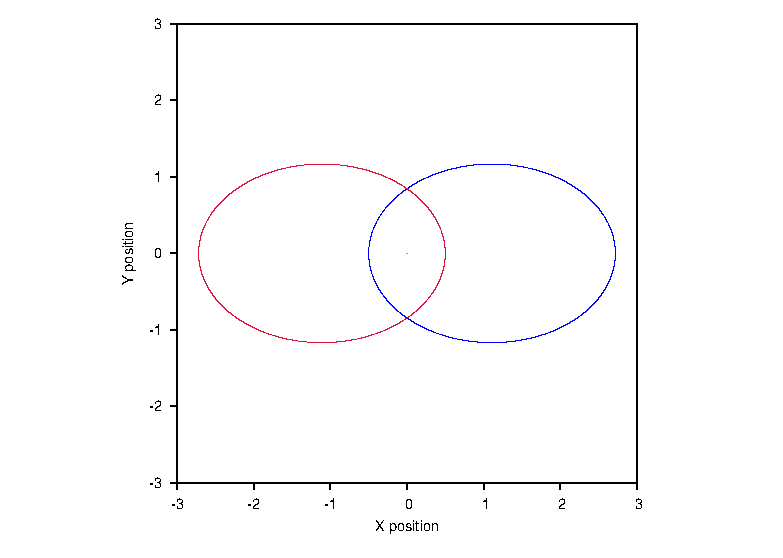
\includegraphics[width=0.9\textwidth]{./results/01-7-01-2/Orbit.eps}
\caption{Configuration 11}
\label{fig:config11}
\end{figure}
\begin{figure}[H]
\centering
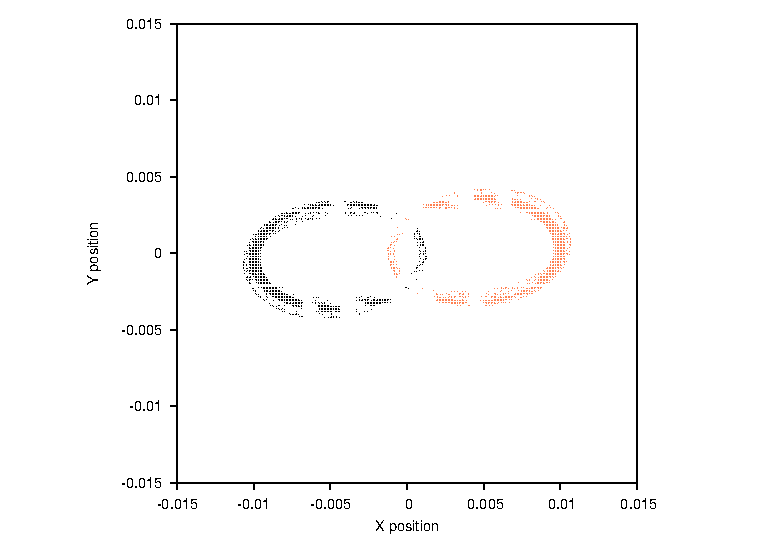
\includegraphics[width=0.9\textwidth]{./results/01-7-01-2/Inner.eps}
\caption{Configuration 11 - Inner Bar}
\label{fig:config11i}
\end{figure}

\begin{figure}[H]
\centering
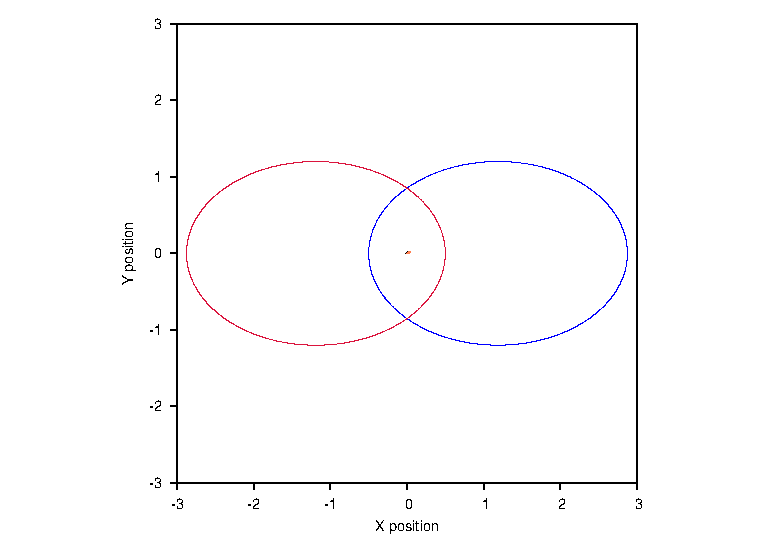
\includegraphics[width=0.9\textwidth]{./results/02-75-02-1/Orbit.eps}
\caption{Configuration 12}
\label{fig:config12}
\end{figure}
\begin{figure}[H]
\centering
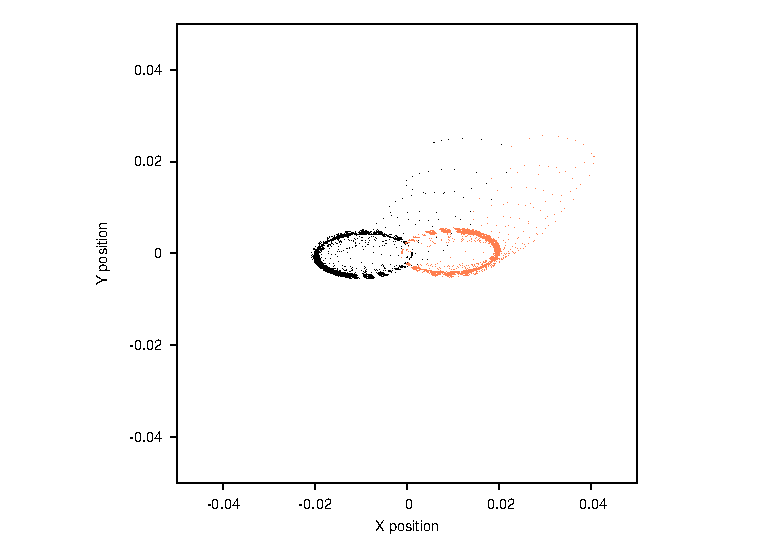
\includegraphics[width=0.9\textwidth]{./results/02-75-02-1/Inner.eps}
\caption{Configuration 12 - Inner Bar}
\label{fig:config12i}
\end{figure}

\begin{figure}[H]
\centering
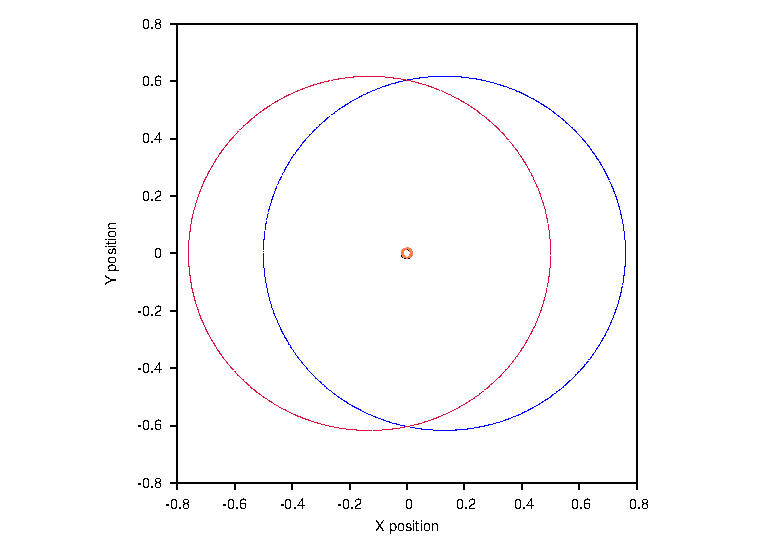
\includegraphics[width=0.9\textwidth]{./results/025-65-02/Orbit.eps}
\caption{Configuration 13}
\label{fig:config13}
\end{figure}
\begin{figure}[H]
\centering
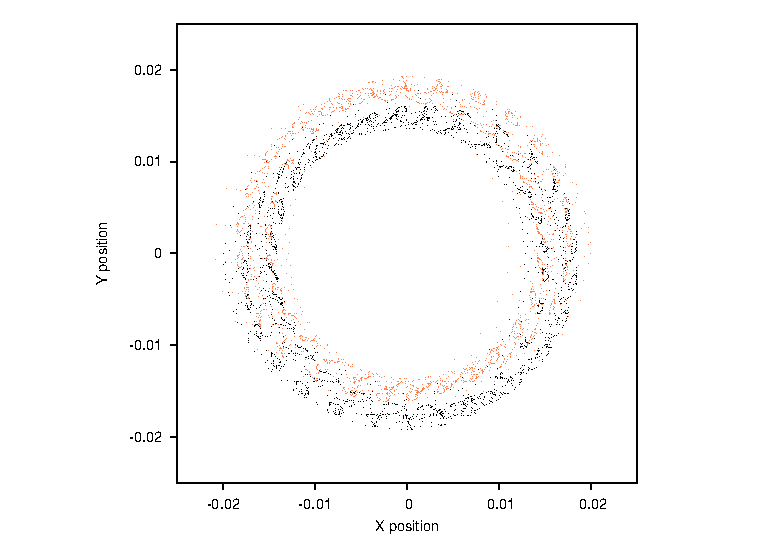
\includegraphics[width=0.9\textwidth]{./results/025-65-02/Inner.eps}
\caption{Configuration 13 - Inner Bar}
\label{fig:config13i}
\end{figure}

\begin{figure}[H]
\centering
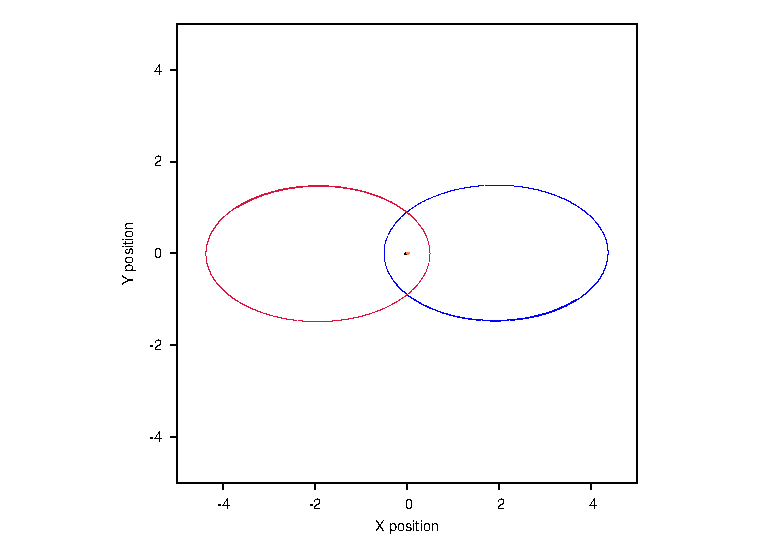
\includegraphics[width=0.9\textwidth]{./results/05-9-05-1/Orbit.eps}
\caption{Configuration 14}
\label{fig:config14}
\end{figure}
\begin{figure}[H]
\centering
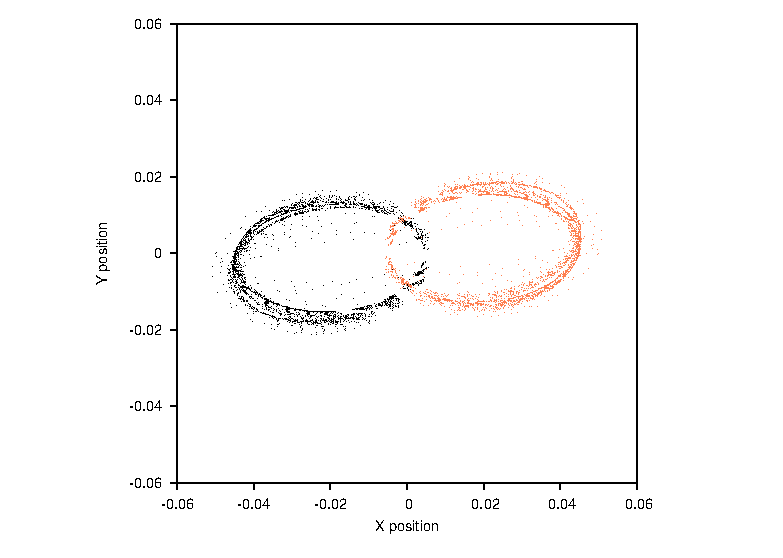
\includegraphics[width=0.9\textwidth]{./results/05-9-05-1/Inner.eps}
\caption{Configuration 14 - Inner Bar}
\label{fig:config14i}
\end{figure}

\begin{figure}[H]
\centering
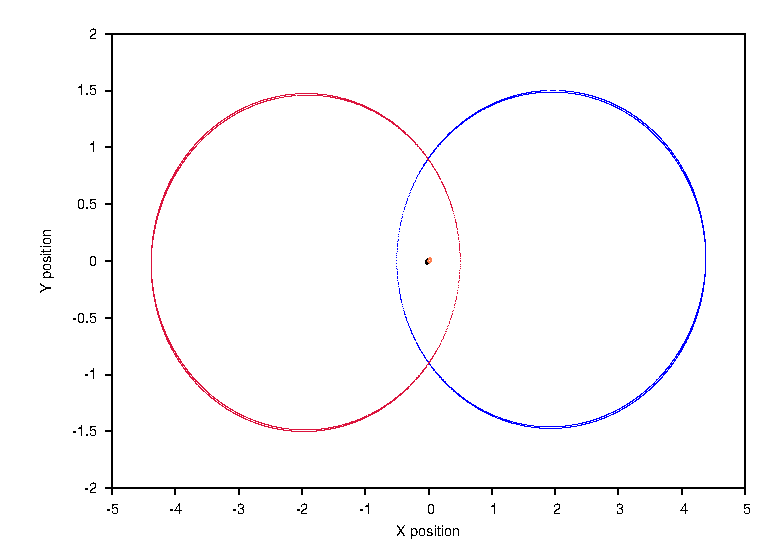
\includegraphics[width=0.9\textwidth]{./results/05-9-05-15/Orbit.eps}
\caption{Configuration 15}
\label{fig:config15}
\end{figure}
\begin{figure}[H]
\centering
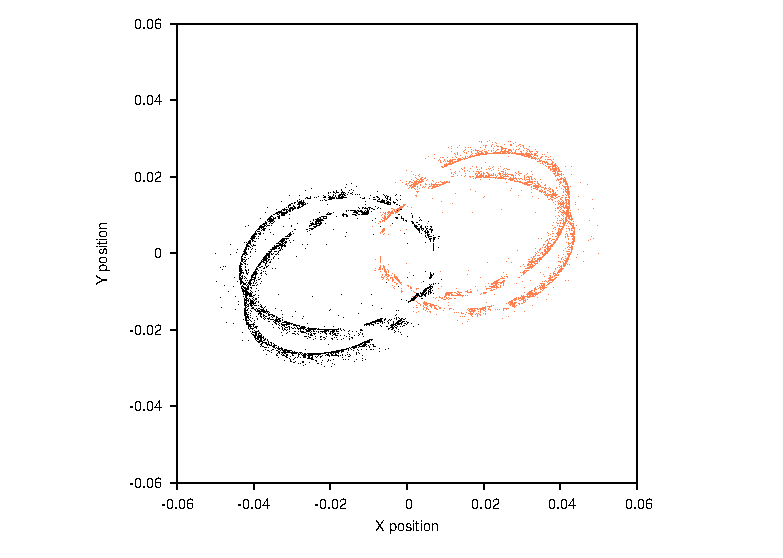
\includegraphics[width=0.9\textwidth]{./results/05-9-05-15/Inner.eps}
\caption{Configuration 15 - Inner Bar}
\label{fig:config15i}
\end{figure}

\begin{figure}[H]
\centering
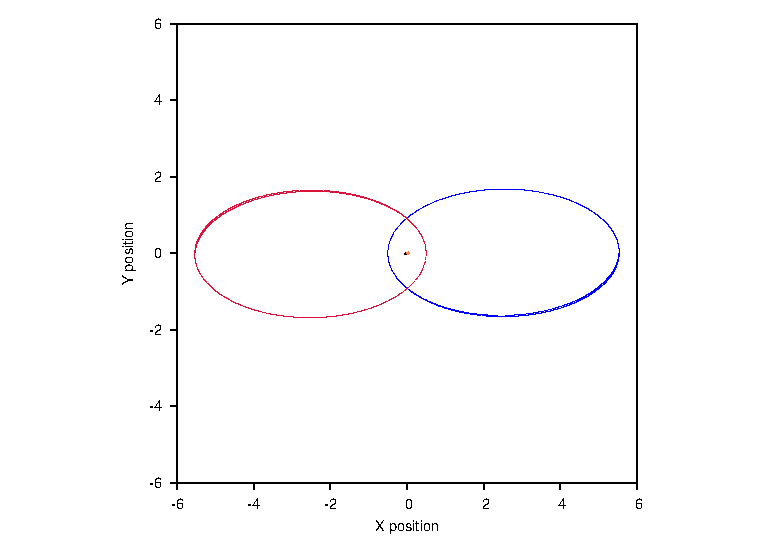
\includegraphics[width=0.9\textwidth]{./results/06-95-06-15/Orbit.eps}
\caption{Configuration 16}
\label{fig:config16}
\end{figure}
\begin{figure}[H]
\centering
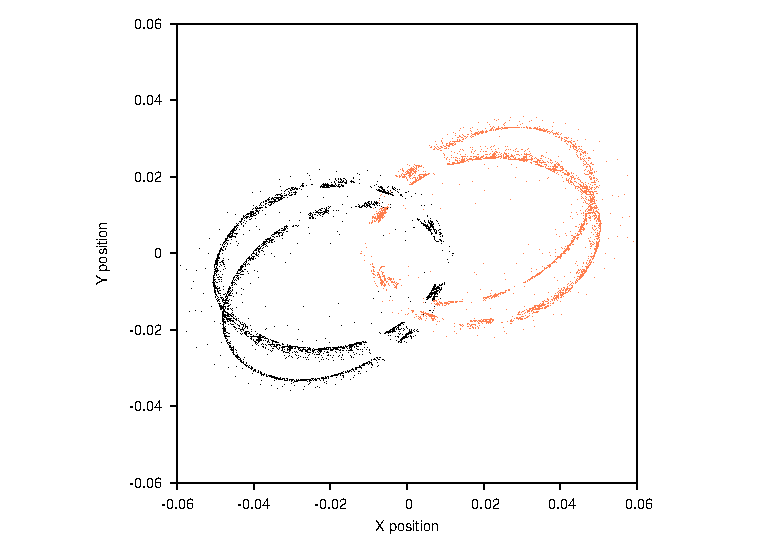
\includegraphics[width=0.9\textwidth]{./results/06-95-06-15/Inner.eps}
\caption{Configuration 16 - Inner Bar}
\label{fig:config16i}
\end{figure}

\begin{figure}[H]
\centering
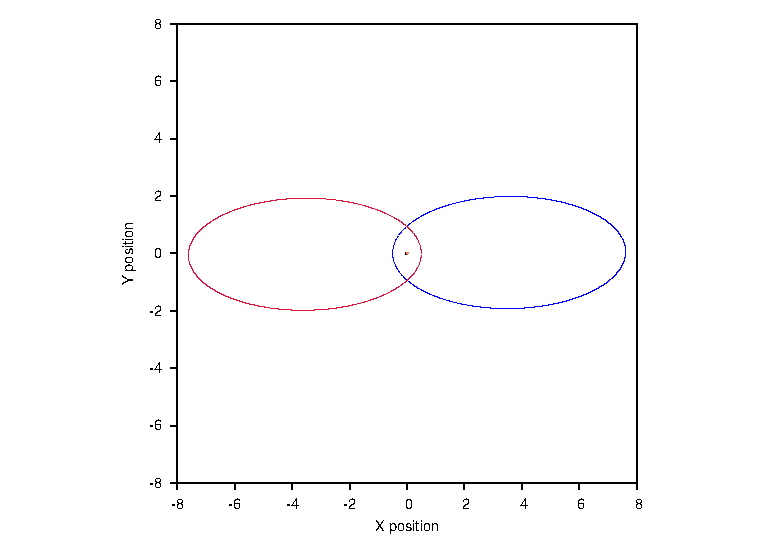
\includegraphics[width=0.9\textwidth]{./results/07-1-07-15/Orbit.eps}
\caption{Configuration 17}
\label{fig:config17}
\end{figure}
\begin{figure}[H]
\centering
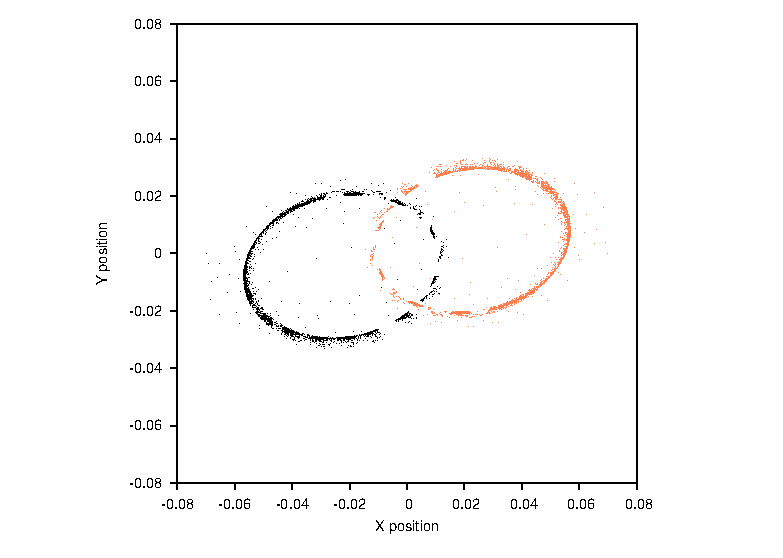
\includegraphics[width=0.9\textwidth]{./results/07-1-07-15/Inner.eps}
\caption{Configuration 17 - Inner Bar}
\label{fig:config17i}
\end{figure}

\begin{figure}[H]
\centering
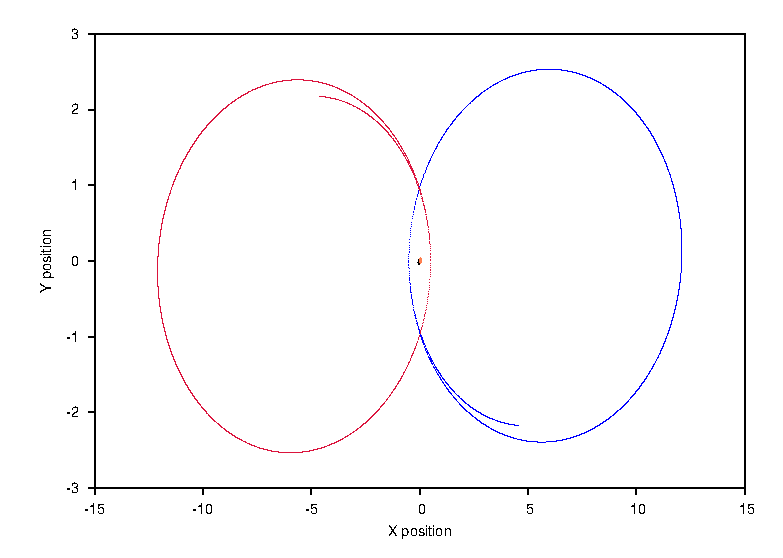
\includegraphics[width=0.9\textwidth]{./results/08-105-08-12/Orbit.eps}
\caption{Configuration 18}
\label{fig:config18}
\end{figure}
\begin{figure}[H]
\centering
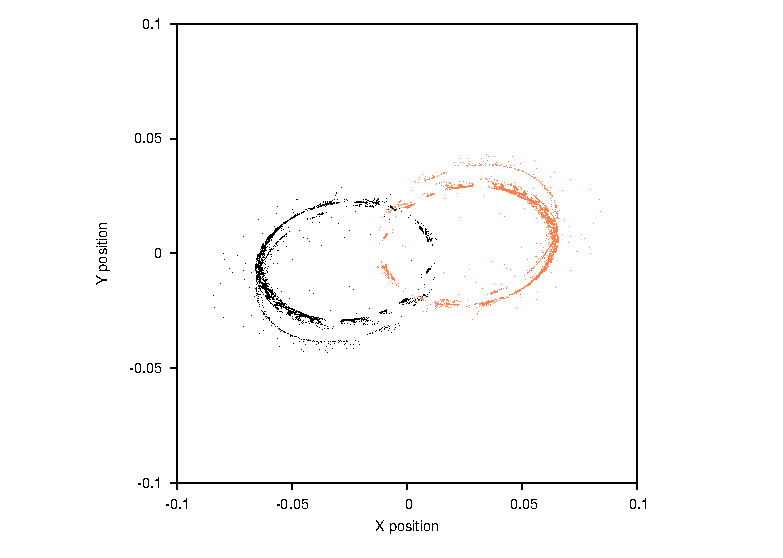
\includegraphics[width=0.9\textwidth]{./results/08-105-08-12/Inner.eps}
\caption{Configuration 18 - Inner Bar}
\label{fig:config18i}
\end{figure}
\end{document}